\chapter{Evaluation der Ergebnisse}\label{evaluation}

Im Folgenden werden die entwickelten Modelle untersucht und evaluiert. Für die beiden \acl{RF}s wird die Implementierung von \texttt{sklearn} genutzt, für die Gradient Boosted Trees die Bibliothek \texttt{XGBoost}, da das \ac{XGB} besser ist als die in \texttt{sklearn}.\footcite[Kapitel 10]{Harrison2019} Die Ergebnisse der Modelle werden sowohl für das reduzierte als auch das vollständige Merkmalsset berechnet, verglichen und aufbauend darauf die Merkmalsauswahl optimiert. Außerdem wird der Einfluss der gewählten Segmentlänge und des gewählten Schwellwertes der Annotation untersucht. Für alle Untersuchungen wird das gleiche Testset wie in Kapitel \ref{analyse} verwendet.

\section{Modellevaluation} %TODO: besserer Titel? Merkmalsauswahl?

Zunächst werden alle Modelle sowohl mit dem vollständigen Merkmalsset als auch dem reduzierten Merkmalsset verglichen, siehe Tabelle \ref{fig:comparison-all}. Die Ergebnisse der Klassifikation mit Gradient Boosted Trees und \acl{RF}s sind zunächst ähnlich. Bei der Regression erreichen Gradient Bossted Trees eine sehr hohe Coverage von über 80\,\% mit einem zu den anderen Modellen verhältnismäßig hohen \ac{MAE} von über 16\,\si{FE}. Insgesamt zeigt sich bereits, dass eine deutlich höhere Coverage als bei der reinen Betrachtung der Intervallschätzer des CLIE-Algorithmus erreicht wird. Diese lag beispielsweise für $q\textsubscript{th} = 0.3$ bei 20,93\,\% mit einem \ac{MAE} von 13,90\,\si{FE}.

	\begin{table}[H]
	\centering
		\begin{tabular}{l | l | l|| c | c | c | c }
 						& Merkmalsset	& Modell			& \ac{MAE} [FE]	& Coverage [\%]	& F1-Score	& AUC	\\ \hline
 		\multicolumn{3}{l ||}{insgesamt}					& 21{,}85		& -				& - 		& -		\\
 		\multicolumn{3}{l ||}{annotiert}					& 3{,}28			& 43{,}21		& - 		& -		\\ \hline
 		\multirow{4}{*}{Klassifikation}
 						& \multirow{2}{*}{reduziert}		
 										& \acs{RF} 		& 13{,}87		& 32{,}09		& 0{,}54	& 0,69	\\
 						&				& \acs{XGB}		& 14{,}60		& 38,10			& 0{,}56	& 0,68	\\\cline{2-7} %TODO: update numbers
 						& \multirow{2}{*}{alle}
 									 	& \acs{RF}		& 12{,}11		& 36,81			& 0{,}61	& 0,75	\\
 						&				& \acs{XGB} 	& 11,38			& 35,93			& 0,62		& 0,75\\\hline
 		\multirow{4}{*}{Regression}
 						& \multirow{2}{*}{reduziert}
 										& \acs{RF}		& 14,34			& 41,21			& 0,57		& 0,69	\\
 						&				& \acs{XGB}		& 17,79			& 80,77			& 0,63		& 0,69	\\\cline{2-7}
 					 	& \multirow{2}{*}{alle}		
 					 					& \acs{RF}		& 12,56			& 46,27			& 0,64		& 0,75\\
 					 	&				& \acs{XGB} 		& 16,04			& 81,80			& 0,65		& 0,74\\
		\end{tabular}
		\caption{Vergleich der aller Modelle mit reduziertem und vollständigem Merkmalsset}
		\label{fig:comparison-all}
	\end{table}

Des Weiteren zeigt sich, dass das reduzierte Merkmalsset entgegen der Erwartungen zu etwas schlechteren Ergebnissen führt. Eine Betrachtung der Wichtigkeit der Merkmale für die Modelle mit vollständigem Merkmalsset zeigt, dass für das vollständige Merkmalsset jeweils $\text{ratio}\textsubscript{acf}$ und $\text{ratio}\textsubscript{acf}$ zu den wichtigsten Merkmalen gehören, die beide aussortiert wurden. In Abbildung \ref{fig:rf-clf-all-importances} ist die Verteilung der Relevanz der Merkmale gezeigt. Ein Test mit einem \ac{RF}-Klassifikator mit dem reduzierten Merkmalsset zuzüglich den oben genannten Merkmalen zeigt, dass sich die Performance im Vergleich zum vollständigen Merkmalsset so vergleichbar ist und eine \ac{MAE} von 11,97\,\si{FE} bei einer Coverage von 36,51\,\% erreicht wird.
\begin{figure}[H]
	\centering
	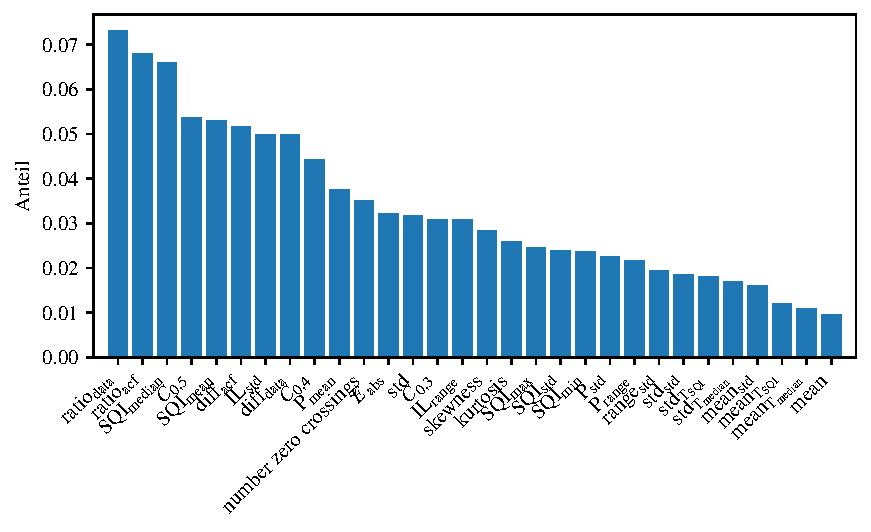
\includegraphics{pic/rf-clf-all-importances.pdf}
 	\caption{Wichtigkeit der Merkmale des \ac{RF}-Klassifikators mit vollständigem Merkmalsset}
 	\label{fig:rf-clf-all-importances}
\end{figure}

Bei den folgenden Untersuchungen wird deshalb das erweiterte reduzierte Merkmalsset verwendet. Die Ergebnisse der 4 Modelle sind in Tabelle \ref{fig:final-results-comparison} abgebildet. Alle vier erzielen ähnliche Ergebnisse, wobei die Regressionsmodelle eine etwas höhere Coverage erreichen. Es gibt im Gegensatz zu den Ergebnissen bei der Verwendung aller Merkmale keine Ausreißer. Sowohl bei Regression als auch Klassifikation erreichen die \ac{XGB}-Modelle bei ähnlichem Fehler eine etwas höhere Coverage. Die \ac{AUC} zeigt, dass alle Modelle bei den gegebenen Daten in der Lage sind, informatives und nicht informatives Signal zu separieren.
%\begin{multicols}{2}
%\begin{itemize}
%	\item Mittelwert
%	\item Kurtosis
%	\item Schiefe
%	\item $\text{diff}\textsubscript{acf}$
%	\item $\text{diff}\textsubscript{data}$
%	\item $\text{ratio}\textsubscript{acf}$
%	\item $\text{ratio}\textsubscript{data}$
%	\item $\text{SQI}\textsubscript{std}$
%	\item $\text{SQI}\textsubscript{min}$
%	\item $\text{SQI}\textsubscript{median}$
%	\item $\text{P}\textsubscript{range}$
%	\item $\text{P}\textsubscript{mean}$
%	\item $\text{mean}\textsubscript{T\textsubscript{median}}$
%	\item $\text{std}\textsubscript{T\textsubscript{median}}$
%	\item $\text{mean}\textsubscript{T\textsubscript{SQI}}$
%	\item $\text{std}\textsubscript{T\textsubscript{SQI}}$
%	\item $\text{IL}\textsubscript{std}$
%	\item $\text{mean}\textsubscript{std}$
%	\item $C_{0,5}$
%	\item $C_{0,4}$
%	\item $C_{0,3}$
%\end{itemize}
%\end{multicols}

\begin{table}[H]
	\centering
	\begin{tabular}{l | l || c | c | c | c }
									& Modell			& \ac{MAE} [FE]	& Coverage [\%]	& F1-Score	& AUC	\\ \hline
 	\multicolumn{2}{l ||}{insgesamt}					& 21{,}85		& -				& - 		& -		\\
 	\multicolumn{2}{l ||}{annotiert}					& 3{,}28			& 43{,}21		& - 		& -		\\ \hline
 	\multirow{2}{*}{Klassifikation}
 									& \acs{RF} 		& 11,97			& 36,51			& 0,61		& 0,75	\\
 									& \acs{XGB}		& 12,44			& 41,99			& 0,64		& 0,74	\\\hline %TODO: update numbers
 	\multirow{2}{*}{Regression}
 									& \acs{RF}		& 12,52			& 46,05			& 0,64		& 0,75	\\ %TODO: update numbers
 									& \acs{XGB}		& 12,44			& 47,59			& 0,63		& 0,74	\\\hline %TODO: update numbers
 	\end{tabular}	
	\caption{Vergleich der aller Modelle mit finalem Merkmalsset}
	\label{fig:final-results-comparison}
	\end{table}

	
Betrachtet man die Wichtigkeit der Merkmale der beiden Klassifikationsmodelle, fällt auf, dass bei dem \ac{XGB}-Klassifikator ein Merkmal allein deutlich wichtiger als alle anderen ist, sowohl beim reduzierten als auch beim vollständigen Merkmalsset. Bei den \ac{RF}-Modellen dagegen, ist die Wichtigkeit gleichmäßiger verteilt. Der direkte Vergleich ist in Abbildung \ref{fig:importances-comparison-rf-xgb-clf} zu sehen. Trotz der unterschiedlichen Gewichtung der Merkmale erzielen beide Modelle ähnliche Ergebnisse. Allerdings ist der \ac{XGB}-Klassifikator weniger stabil für Verzerrung in dem mit Abstand wichtigstem Merkmal $C_{0.5}$. Es zeigt aber auch, dass die Ähnlichkeit der Intervallschätzer des \ac{CLIE}-Algorithmus ein gutes Kriterium zur Beurteilung der Signalqualität ist.

 \begin{figure}[h]
 	\centering
		\begin{subfigure}{.49\textwidth}
			\centering
 			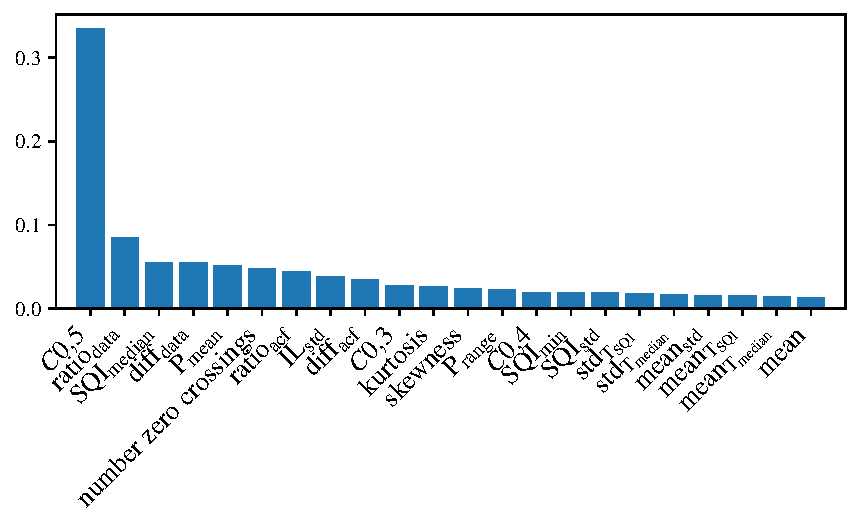
\includegraphics[width=\textwidth]{pic/xgb-clf-final-importances.pdf}
 			\caption{\ac{XGB}-Klassifikator}
 		\end{subfigure}
    	\begin{subfigure}{.49\textwidth}
    		\centering
 			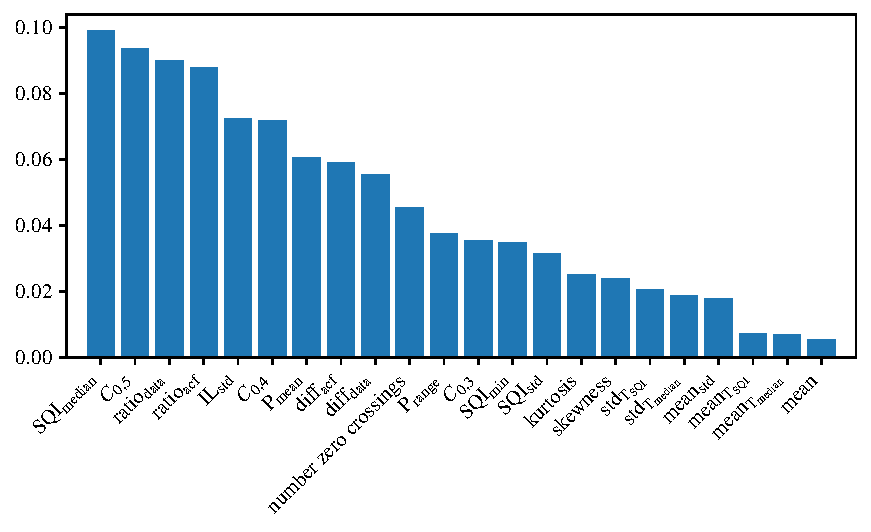
\includegraphics[width=\textwidth]{pic/rf-clf-final-importances.pdf}
 			\caption{\ac{RF}-Klassifikator}
 		\end{subfigure}
 	\caption{Vergleich der Wichtigkeit der Merkmale zwischen \ac{RF}-Klassifikator und \ac{XGB}-Klassifikator}
 	\label{fig:importances-comparison-rf-xgb-clf}
 \end{figure}

Bei der Betrachtung der Regressionsmodelle zeigt sich, dass es bei dem \ac{XGB}-Regressor zwei Merkmale gibt, die bedeutend wichtiger als der Rest sind: Erneut $C_{0,5}$ und $\text{ratio}\textsubscript{data}$. Das \ac{RF}-Modell zeigt erneut eine gleichmäßigere Verteilung der Wichtigkeit der Merkmale. Die Wichtigkeit der übrigen Merkmale ist, wie in Abbildung \ref{fig:importances-comparison-rf-xgb-regr} zu sehen, ähnlich verteilt.

 \begin{figure}[h]
 	\centering
		\begin{subfigure}{.49\textwidth}
			\centering
 			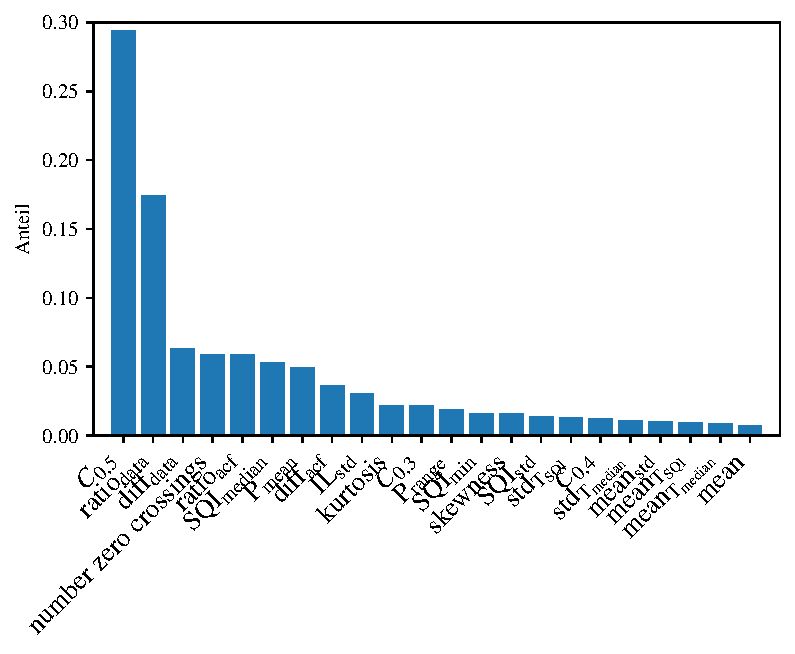
\includegraphics[width=\textwidth]{pic/xgb-regr-final-importances.pdf}
 			\caption{\ac{XGB}-Regressor}
 		\end{subfigure}
    	\begin{subfigure}{.49\textwidth}
    		\centering
 			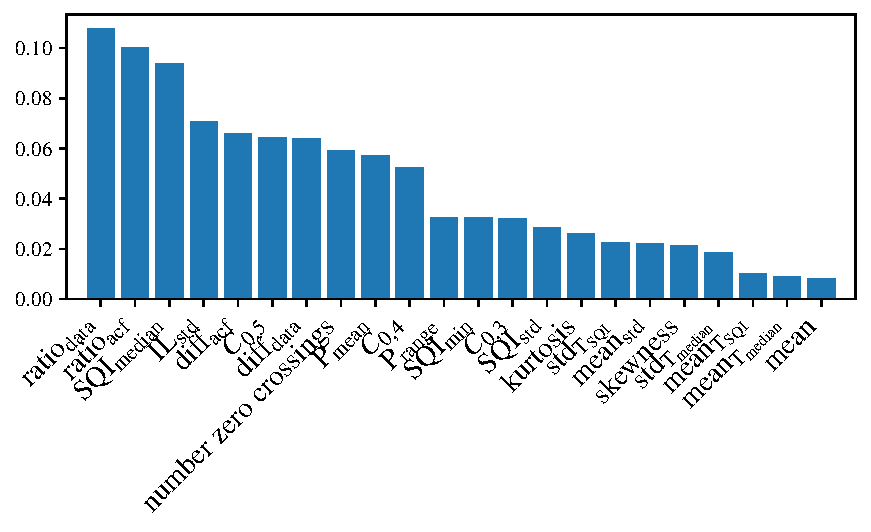
\includegraphics[width=\textwidth]{pic/rf-regr-final-importances.pdf}
 			\caption{\ac{RF}-Regressor}
 		\end{subfigure}
 	\caption{Vergleich der Wichtigkeit der Merkmale zwischen \ac{RF}-Regressor und \ac{XGB}-Regressor}
 	\label{fig:importances-comparison-rf-xgb-regr}
 \end{figure}
 
 Die \ac{RF}-Modelle gewichten die einzelnen Merkmale bei den vorliegenden Daten ähnlicher als die \ac{XGB}-Modelle. Dennoch sind die Ergebnisse der ersten Evaluation ähnlich. Auch ist die Wichtigkeit der Merkmale zwischen den Klassifikations- und Regressionsmodellen ähnlich. Insgesamt zeigen die Regressionsmodelle aber eine überlegende Performance. Eine genauere Evaluation der Coverage und der Verteilung von $E\textsubscript{HR}$ wird für den \ac{RF}-Regressor durchgeführt. Zum Vergleich werden die Ergebnisse der Klassifizierung anhand der Intervallschätzer des \ac{CLIE}-Algorithmus für $q\textsubscript{th}=0{,}3$ und $c\textsubscript{th}$ gezeigt, da mit diesen Schwellwerten ebenfalls eine Reduzierung des \ac{MAE} mit einer vergleichbaren Coverage von 37,87\,\% erreicht wurde. Der Vergleich der erreichten Coverage unter einem bestimmten $E\textsubscript{HR}$, sichtbar in Tabelle \ref{fig:own-coverage-default}, zeigt deutlich, dass die Coverage geringer Fehler deutlich erhöht werden konnte. 
 
  \begin{table}[h]
 	\centering
  	\begin{tabular}{l || c | c | c}
 											& insgesamt 		& \ac{RF}-Regressor & \ac{CLIE}-Intervallschätzer\\\hline
 		$E\textsubscript{HR} < 5$\,\si{FE} 	&  32{,}61\,\% 	& 23,79\,\% 			& 18,32\,\%\\
 		$E\textsubscript{HR} < 10$\,\si{FE} 	&  43{,}21\,\% 	& 28,67\,\% 			& 21,34\,\%\\
 		$E\textsubscript{HR} < 15$\,\si{FE} 	&  51{,}64\,\% 	& 32,02\,\% 			& 23,35\,\%\\
 		$E\textsubscript{HR} < 20$\,\si{FE} 	&  59{,}38\,\% 	& 34,86\,\% 			& 25,12\,\%\\
 	\end{tabular}
 	\caption[Coverage unter bestimmten Fehlern $E\textsubscript{HR}$ nach Klassifikation mittels \ac{RF}-Regressor]{Coverage unter bestimmten Fehlern $E\textsubscript{HR}$ nach Klassifikation mittels \ac{RF}-Regressor}
 	\label{fig:own-coverage-default}
 \end{table}
 
 Auch eine Untersuchung der Verteilung von $E\textsubscript{HR}$ auf den als informativ klassifizierten Segmenten zeigt im Verglich, dass der Anteil des Signals mit einem Fehler $E\textsubscript{HR} > 20\si{FE}$ stark gesenkt werden konnte. Auch liegt der durchschnittliche \ac{MAE} der falsch-negativen Segmente bei xxx\,\si{FE}, was über dem Durchschnitt aller als informativ klassifizierten Segmente von 3,28\,\si{FE} liegt.
 
 \begin{figure}[h]
 	\centering
		\begin{subfigure}{.45\textwidth}
			\centering
 			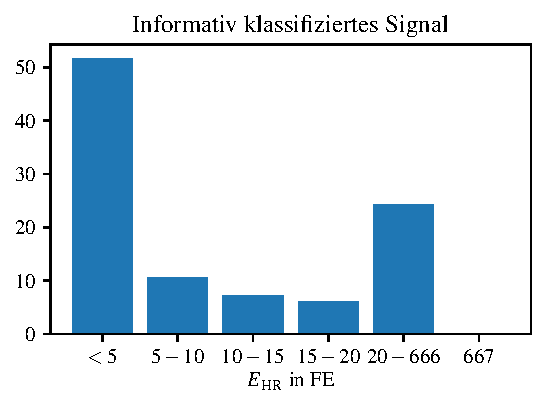
\includegraphics[scale=0.7]{pic/rf-own-final-10-positives.pdf}
 			\caption{\ac{RF}-Regressor}
 		\end{subfigure}
    	\begin{subfigure}{.45\textwidth}
    		\centering
 			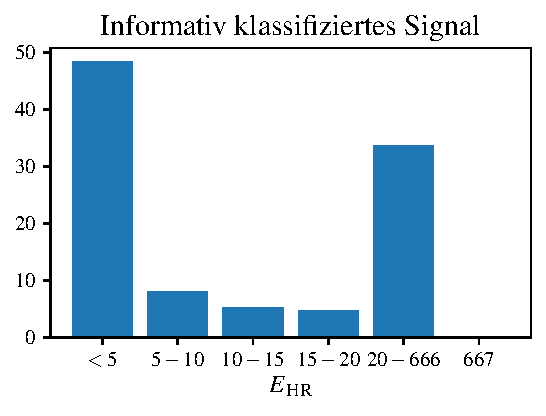
\includegraphics[scale=0.7]{pic/brueser03-positives.pdf}
 			\caption{Ähnlichkeit der Intervallschätzer}
 		\end{subfigure}
 	\caption{Verteilung von $E\textsubscript{HR}$ bei den als informativ klassifizierten Segmenten}
 	\label{fig:own-10-positives}
 \end{figure}
 
 Mit den im Rahmen dieser Arbeit entwickelten Modellen kann also die Signalqualität zuverlässiger als bisher beurteilt werden. Die Coverage durch die Klassifikation konnte erhöht und der \ac{MAE} der als informativ klassifizierten Segmente gesenkt werden.

\section{Einfluss des Schwellwertes der Annotation}

Nachdem die generelle Performance der Modelle untersucht wurde, wird nun der Einfluss des verwendeten Schwellwertes der Annotation untersucht.

\section{Einfluss der Segmentlänge}



